\documentclass{tufte-handout}
\usepackage{graphicx}
\graphicspath{ {./images/} }

\title{Deep Learning and CNNs}
\author{Andr\'es Ponce}

\begin{document}
\maketitle

\begin{abstract}
Deep Learning methods allow us to perform other functions such as 
object recognition obtained from image datasets.
\end{abstract}

\section{Conventional Approach to Object Recognition}
The key steps in object recognition involve \textbf{feature extraction}
from several images. However, features may look different when recognizing 
different types of objects.

We could have a mdoel with \textbf{hand-crafted} feature detection. Here, we could
define by hand the kind of features we would like to see in our model. After we go through
the feature extractor we could have a simple classifier. 

Another approach is instead to have a \textbf{trainable feature extractor}, 
along with a trainable classifier.

\section{Neural Networks}
If we recall, \textbf{neural networks} are a series of layers, composed of individual 
\textbf{neurons} and which connect and communicate to neurons the layer before or after it.

\begin{marginfigure}
	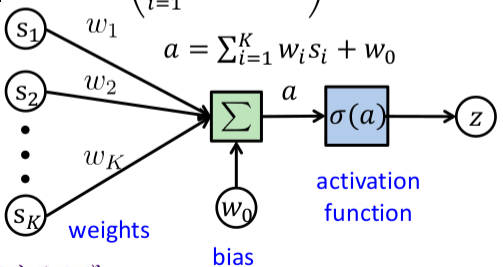
\includegraphics[scale=0.3]{NNs}
	\caption{In neural networks, we have a set $\mathbf{s}$ of input values, which are then 
		summed up through the different layers. Afterwards, we pass it through an 
	\textbf{activation function} $\sigma(a)$, which then leads to the class we predict it into.
	}
\end{marginfigure}

\textbf{Training} the neural network consists in trying to minimzize the loss function. 
For classification, the loss function might be the distance between the correct classification
	and our predicted values.
The formula might look something like:
\[ L(\theta) = \sum_{i=1}^{N}\|\mathbf{y}_{i} -  g_{w}(\mathbf{x_{i}})\|^{2}\]

To minimize it, we use the technique called \textbf{gradient descent}. 
This technique involves finding the values for which the \textbf{derivative} of the loss function decreases. 
Even within gradient descent, there are some different types we might wish to use. 
For example, \textbf{steepest descent} uses batch processing to change the parameter vector $\mathbf{w}$.
\footnote{Remember batch methods operate on the whole training set to modify weights.}

Another method for gradient descent involves selecting a subset of the dataset to use when measuring 
	error.
This is called \textbf{stochastic} gradient descent. 
Here we use a formula such as 
\[E(w) = \frac{1}{2}\sum_{n=1}^{N}\{y(x_{n}, w) - t_{n}\}^{2}\]
also known as \textbf{sum of squares}.
\footnote{Sum of squares errors are more useful for problems resembling regression.}
\begin{marginfigure}
	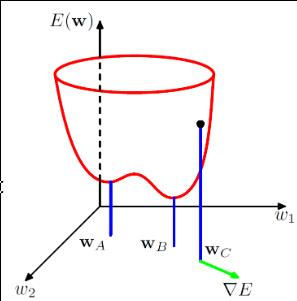
\includegraphics[scale=0.3]{gradient_descent}
	\caption{Visual representation of gradient descent. We are trying to find the global
		minimum of the error function, by following the gradient ``down" into the global 
		minimum.}
\end{marginfigure}

Calculating the error at every single node each iteration may be too intensive to repeat at every step,
	so insted we can calculate the error via an algorithm called \textbf{backpropagation}.
The backpropagation algorithm serves us to calculate the error in the nodes. 
Remember the value of
the activaiton function is a function of the weights of the layers incoming, so something like:
\[ a_{j} = \sum_{i=1}^{D}w^{(1)}_{ji}x_{i} + w_{j0}^{(1)}\]

There are a couple of steps for calculating the error:
\begin{enumerate}
	\item Calculate the error for each of the $k$ classes. This is done for each output layer.
			\[ \delta_{k} = y_{k} - t_{k}\]
	\item Calculate the error for the \textbf{hidden layers}. We use the formula
			\[ \delta_{j} = h'(a_{j})\sum_{k}^{}w_{kj}^{(2)}\delta_{k}\]
				Remember $h(a)$ is the function which further modifies the activation function $a$ of
				each neuron in the hidden layer.
				\footnote{Still have some steps missing.}
\end{enumerate}
\subsection{What is a Deep Neural Network?}
Essentially it is a neural network with many hidden layers.
\footnote{Deep, get it?}

We have multiple different possible architectures for neural networks.
%\begin{centering}
%
%\begin{figure}
%		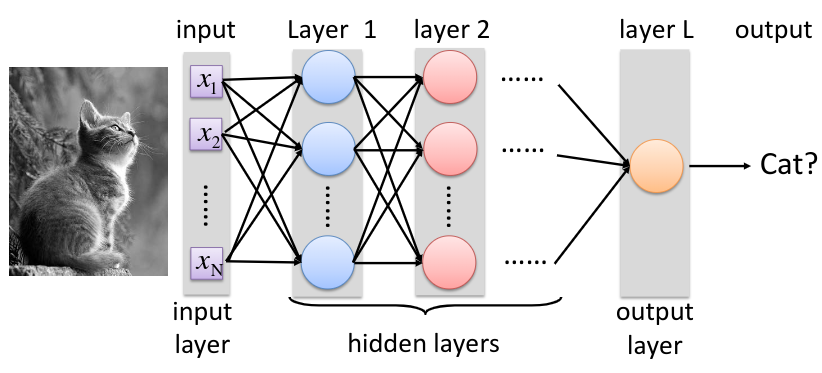
\includegraphics[scale=0.3]{obj_recognition}
%		\caption{Architecure of deep learning for object recognition.}
%\end{figure}
%\end{centering}

For object recognition such as pictured above, we can model an image just as a grid of pixel values.
Then we can use the values as input to the neural network. 
However, for a $n x m$ image, we would need to have $(n x m)^{l}$ total connetions, where $l$ is
	the number of layers in our network
Thus we can use \textbf{Convolutional Neural Networks} for help with this.

\subsection{Convolutional Neural Networks}
A convolutional neural network is a multi-layer neural network with \textbf{local connectivity}
	and \textbf{weight-sharing}.
	\subsection{Local Connectivity}
The main idea of a CNN is that a normal neural network does not scale that well when applied to
	larger and larger inputs such as images.
So we instead map a \textit{region} of the input image to a given neuron in a convolution layer.
This is due to the fact that a given pixel in an image will likely be of use in its local region rather
	than in the entire image. 
Thus having a fully connected network would most likely have a lot of overfitting or simply unimportant weights.
This would reduce the number of parameters we need in our model.

Once we take a section of the image as a neuron, we have what's called a \textbf{convolutional layer}.
\subsection{Weight Sharing}
We can usually calculate the weight over several layers of information. 

\begin{marginfigure}
		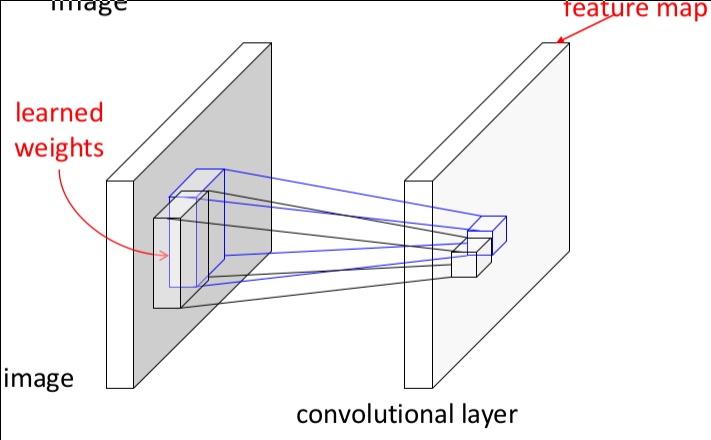
\includegraphics[scale=0.2]{weight_sharing}
	\caption{Weight sharing among various small regions of the input image.}
\end{marginfigure}

We have a couple aspects we want to focus on:
\begin{itemize}
	\item \textbf{Input layer}: The input layer contains $n$ rows and $m$ columns. The input also contains 
			\textbf{depth} information, maybe like pixel color values.
	\item \textbf{Convolutional Layer}: We compute the dot product between the image values and the weights 
			in the connected region. 
	\item \textbf{Pool Layer}: The pool layer performs downsampling along some of the dimensions of the 
			input.
	\item \textbf{Fully Connected Layer}: The final layer which is used to determine the class output. 
			Similar to a regular NN, every node in layer $j$ is connected to every node in the previous
					layer.
\end{itemize}
Once we take the image and pass it through the convolutional layer, we can pass it through several 
	\textbf{filters}. 
These filters can apply a different weight to particular portions of the image. 
\footnote{A \textbf{convolution} is a type of function that describes how two different functions are to 
be applied.}
A convolutional layer will then perform convolution and then pass the output through an activation function.
For a map of size $nxn$, and a filter of size $fxf$, we will have a resulting matrix of size $n-f+1$.
\footnote{Since we lose information around the border of the input matrix when performing this process,
	we can do \textbf{zero-padding} aroundt the border to preserve the dimensions.}

Apart from the convolutional layer, we also have the \textbf{pooling layer}.
The pooling layer helps make the dimensions more manageable, and they operate on the feature representatinons
	individually.

Starting from an input image as input, we first might perform several \textbf{convolutions} using different
\textbf{filters}. 
These convolutions are \textit{learned parameters}. 
Then, we perform some spatial pooling by analyzing similar groups of pixels in the image.
Remember that it does not make much sense to have a whole bunch of fully connected layers, since closer 
	pixels don't have that  much relation with faraway pixels.
Thus, if we want to compare general areas of the images, then we could filter the image several times.
\end{document}
